\chapter{SQL Code Generation}
\label{chapter:ocl2sql}

\begin{flushright}
\textit{Chapter written by Bj�rn Freitag}
\end{flushright}

This chapter describes how the SQL Code Generator \keyword{OCL2SQL} provided 
with Dresden OCL can be used. A general introduction into Dresden OCL can 
be found in chapter~\ref{chapter:introduction}. 

Actual the SQL Code Generator is able to generate the following SQL dialects:
\begin{itemize}
  \item Standard SQL
  \item PostgreSQL
  \item Oracle SQL
  \item MySQL
\end{itemize}



\section{Code Generator Preparation}
This chapter uses the \keyword{University Example} which is provided with 
Dresden OCL. The example is show in Figure~\ref{pic:example:university01}. To
import the university example into our Eclipse workspace we have to create a new Project into our workspace (here called 
\model{tudresden.ocl20.pivot.\linebreak[0]examp\-les.\linebreak[0]university}) and
use the import wizard \eclipse{General -> Archive File} to import the example 
provided as a \acs{JAR} archive. In the following window we select the directory
where the \acs{JAR} file is located (probably the \model{plugins} or
\model{dropins} directory inside the Eclipse root folder). We select the archive
\model{tudresden.ocl20.pivot.\linebreak[0]examples.university\_XXX.jar} and push the 
\eclipse{Finish} button (if you use a source code distribution of 
Dresden OCL instead, you can import the project 
\model{tudresden.ocl20.pivot.examples.university} using the import wizard 
\eclipse{General -> Exis\-ting Pr\-ojects into Workspace}).\\

\begin{figure}[!t]
	\centering
	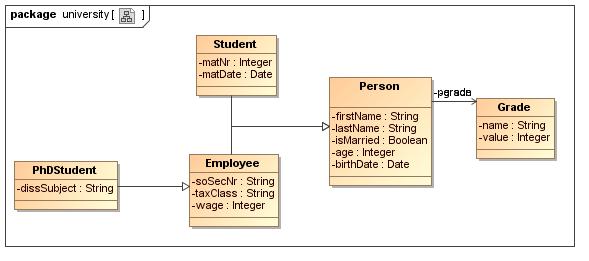
\includegraphics[width=0.85\linewidth]{figures/examples/university01}
	\caption{the UML diagram of the university example.}
	\label{pic:example:university01}
\end{figure}

Now we have imported all files we need to run this tutorial. The project 
provides a model file which contains the university class diagram (the model file is located at 
\model{model/university.uml}) and the constraint file we want to generate code for 
(located at
\model{con\-straints/\linebreak[0]uni\-ver\-si\-ty\linebreak[0].ocl}). One
invariant is shown in Listing~\ref{lst:codegen:universityInvariant}. It is contained in the
constraint file we want to generate code for. The invariant declares, that the
\model{grade} of any \model{Person}'s superviser must be greater thant its own
\model{grade}.

\begin{figure}[!htbp]
  \lstset{
    language=OCL
  }
  \begin{lstlisting}[caption={a simple invariant.}, captionpos=b, label=lst:codegen:universityInvariant]
context Person
inv tudOclInv1: self.supervisor.grade.value > self.grade.value
  \end{lstlisting}
  
\end{figure}



\section{Code Generation}
To prepare the code generation we have to import the model 
\model{model/university.uml} into the \eclipse{Model Browser}. We use the model
import wizard of Dresden OCL to import the model. This procedure is explained in
Chapter~\ref{chapter:introduction}. Afterwards, we have to open the constraint
file \model{con\-straints/\linebreak[0]university.ocl}. After the 
importation, the \eclipse{Model Browser} should look like illustrated in 
Figure~\ref{pic:codegen:modelBrowserSQL}. Now we can start the code generation.
By selecting the item \eclipse{Generate SQL Code} of the menu \eclipse{Dresden
OCL} the sql code generation can be started.

\begin{figure}[!t]
	\centering
	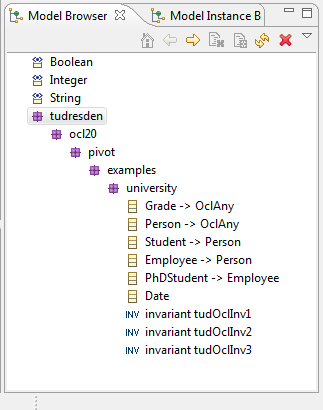
\includegraphics[width=0.6\linewidth]{figures/codegen/modelBrowserSQL}
	\caption{The Model Browser containing the University Model and its Constraints.}
	\label{pic:codegen:modelBrowserSQL}
\end{figure}


\subsection{Selecting a Model}
A wizard opens and we have to select a model for code generation (see 
Figure~\ref{pic:codegen:codegen01SQL}). We select the \model{university.uml} model and
push the \eclipse{Next} button.

\begin{figure}[!p]
	\centering
	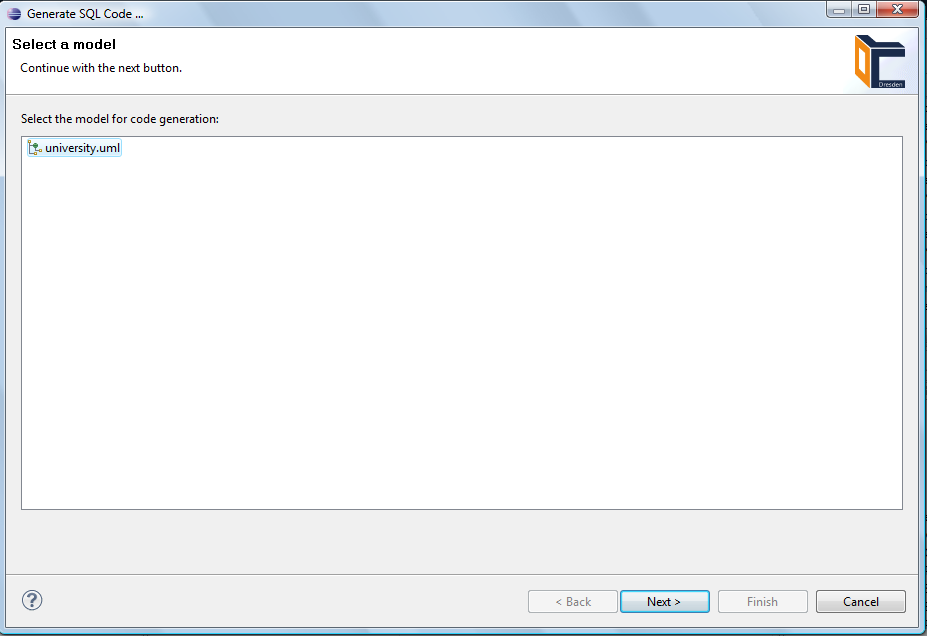
\includegraphics[width=1.0\linewidth]{figures/codegen/codegen01SQL}
	\caption{The first Step: Selecting a Model for Code Generation.}
	\label{pic:codegen:codegen01SQL}

	\vspace{2.0em}
	
	\centering
	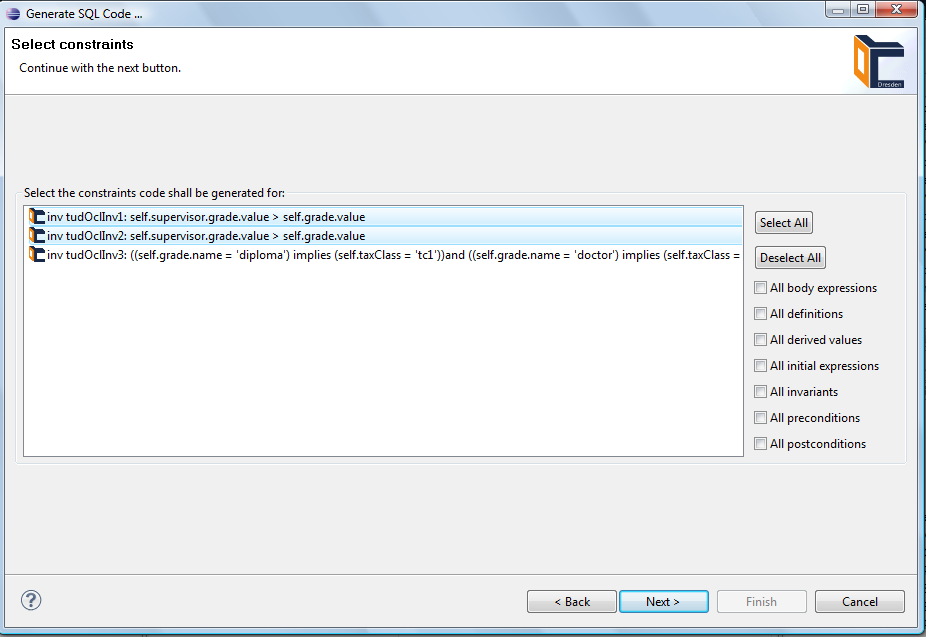
\includegraphics[width=1.0\linewidth]{figures/codegen/codegen02SQL}
	\caption{The second Step: Selecting Constraints for Code Generation.}
	\label{pic:codegen:codegen02SQL}
\end{figure}


\subsection{Selecting Constraints}
As a second step we have to select the constraints we want to
generate code for. We only select the constraints \model{inv: oclInv1} and
\model{inv: oclInv2}. After selecting the constraints we click on the
\eclipse{Next} button (see Figure~\ref{pic:codegen:codegen02SQL}).

\begin{figure}[!t]
	\centering
	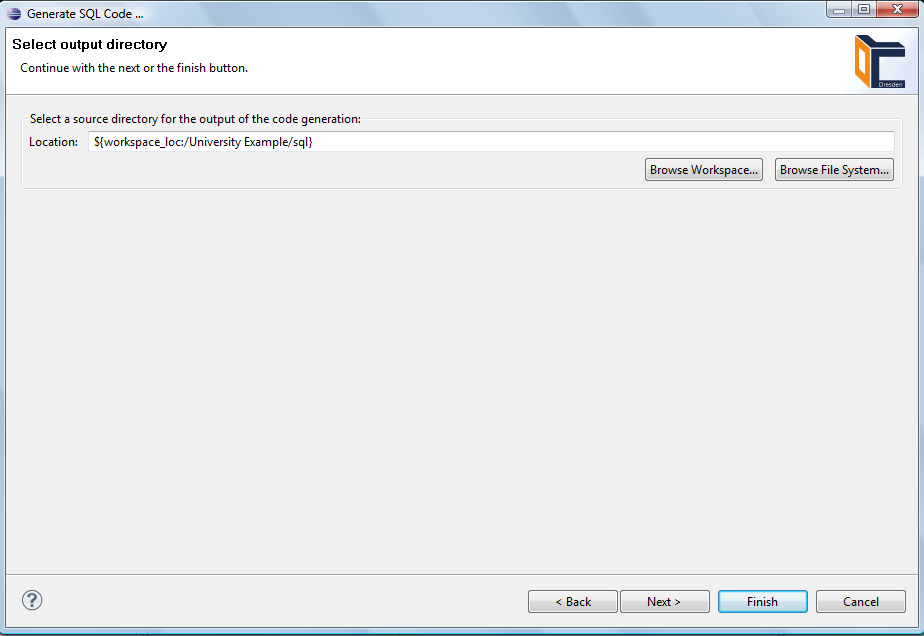
\includegraphics[width=1.0\linewidth]{figures/codegen/codegen03SQL}
	\caption{The third Step: Selecting a target directory for the Generated Code.}
	\label{pic:codegen:codegen03SQL}

	\vspace{2.0em}
	
	\centering
	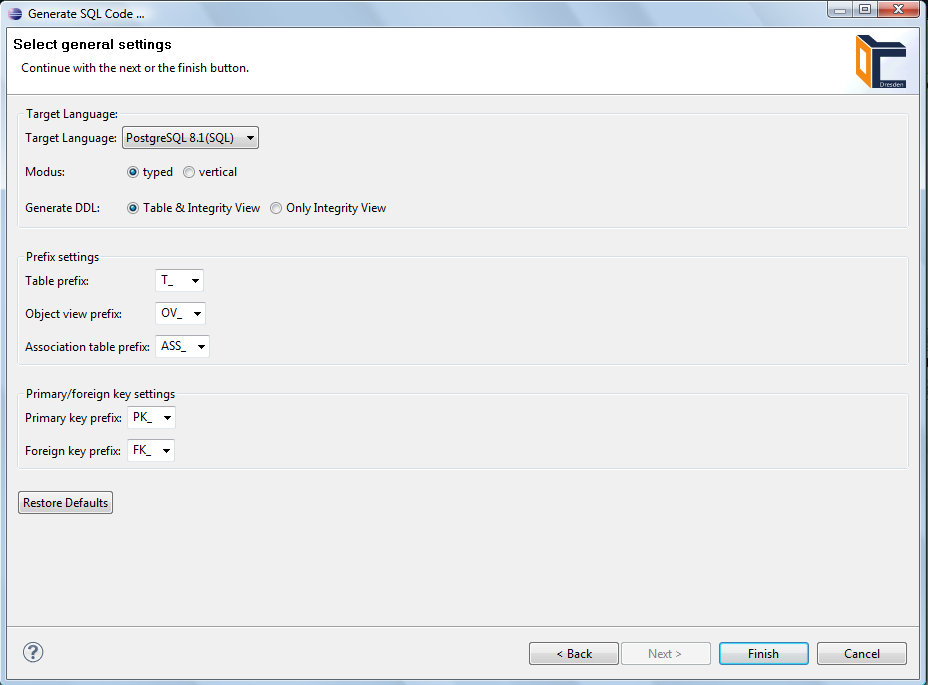
\includegraphics[width=1.0\linewidth]{figures/codegen/codegen04SQL}
	\caption{The fourth Step: General Settings for the Code Generation.}
	\label{pic:codegen:codegen04SQL}
\end{figure}


\subsection{Selecting a target directory}
Now, we have to choice the directory where the generated code will be stored.
We select the folder \model{sql} in this project (which is 
\model{tudresden.\linebreak[0]ocl20.pivot.examples.university/\linebreak[0]sql})
(see Figure~\ref{pic:codegen:codegen03SQL}). We can push the \eclipse{Next} button.

On the following page of the wizard we can specify general settings for the code
generation (see Figure~\ref{pic:codegen:codegen04SQL}). We can choice a SQL
dialect for the generated code. The modus of SQL generation decides how
inheritance relationships are described in the SQL schema. In the typed
modus all subclass properties will be written to the table of the super class.
Any class has its own table with the own properties in the vertical modus. If
you wish only to generate the code for invariant you must choice \model{Only
Integrity View} otherwiese the table schema will be generated as well. The other
parameter will set the prefix for the different parts of the SQL schema. We can
finish the settings and start the code generation with the \eclipse{Finish} button.



\section{The Generated Code}
After finishing the wizard, the code for the selected constraints will be 
generated. To investigate the results it can be necessary to refresh the
project (F5). Our project contains two new SQL files in the folder \eclipse{sql}
(see Figure~\ref{pic:codegen:projectExplorerSQL}). The file 
\eclipse{2010-09-29-09-34\_schema.sql} has the table and view schema of the model. 
Every class of the model has its own view. Over this view the
data(object) of the class can be accesssed. The other file
\eclipse{2010-09-29-09-34\_view.sql} has the views for the invariants (see
Figure~\ref{pic:codegen:generateSQL}). The views contain all objects that
violtate the specific invariant (see Listing~\ref{lst:codegen:sqlInvariant}).

\begin{figure}[!p]
	\centering
	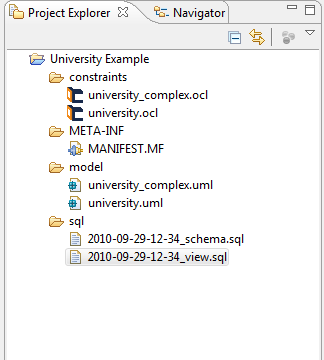
\includegraphics[width=0.45\linewidth]{figures/codegen/projectExplorerSQL}
	\caption{The Package Explorer containing the new SQL code files.}
	\label{pic:codegen:projectExplorerSQL}

	\vspace{2.0em}
	
	\centering
	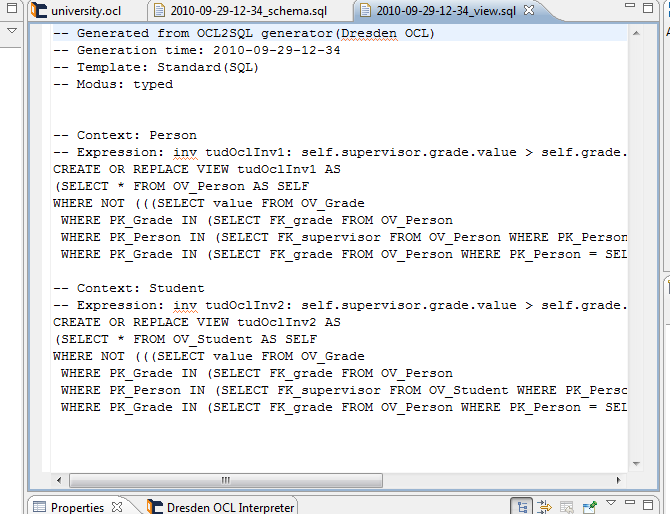
\includegraphics[width=0.45\linewidth]{figures/codegen/generateSQL}
	\caption{The Package Explorer containing the new SQL code files.}
	\label{pic:codegen:generateSQL}

	\vspace{2.0em}
	
 \lstset{
    language=SQL
 }
 \begin{lstlisting}[caption={SQL Code for invariant oclInv1.}, captionpos=b,
  label=lst:codegen:sqlInvariant] -- Context: Person
-- Expression: inv tudOclInv1: self.supervisor.grade.value > self.grade.value
CREATE OR REPLACE VIEW tudOclInv1 AS
(SELECT * FROM OV_Person AS SELF
WHERE NOT (((SELECT value FROM OV_Grade
 WHERE PK_Grade IN (SELECT FK_grade FROM OV_Person
 WHERE PK_Person IN (SELECT FK_supervisor FROM OV_Person WHERE PK_Person = SELF.PK_Person))) > (SELECT value FROM OV_Grade
 WHERE PK_Grade IN (SELECT FK_grade FROM OV_Person WHERE PK_Person = SELF.PK_Person)))));
  \end{lstlisting}
\end{figure}

\section{Summary}
  
How to generate SQL code using the 
\keyword{OCL2SQL} code generator of Dresden OCL was described in this chapter.
Besides the use of \keyword{OCL2SQL} via Dresden OCL's GUI, you can also invoke
OCL2SQL via Dresden OCL's \acs{API}. The easiest way to connect to Dresden OCL
is via its \emph{Facade} providing interfaces for all services of Dresden OCL. 
How to use Dresden OCL's facade is documented in Chapter~\ref{chapter:integration}.
